\section{ПРОЕКТИРОВАНИЕ ВЕБ-ПРИЛОЖЕНИЯ}

\subsection{Анализ целевой аудитории}

Основной целевой аудиторией разрабатываемого веб-приложения являются малые рабочие группы, стартапы, IT-команды на начальном этапе развития и студенческие проектные коллективы. Как правило, численность таких команд составляет от 3 до 20 человек.

В ходе анализа были выявлены основные проблемы (боли) данной аудитории при организации совместной работы традиционными методами:
\begin{itemize}
    \item Потеря информации и артефактов (файлов) при обсуждении рабочих процессов в неспециализированных мессенджерах;
    \item Неочевидность статуса выполнения проекта в целом (отсутствие понимания, какой сотрудник занят конкретной задачей в данный момент);
    \item Высокий порог входа и перегруженность интерфейса в крупных корпоративных системах, что требует излишнего времени на обучение новых сотрудников.
\end{itemize}

Для удовлетворения этих потребностей и обеспечения безопасности системы была спроектирована ролевая модель доступа (RBAC). Исходя из паттернов поведения пользователей, выделены две ключевые роли:
\begin{itemize}
    \item \textbf{Администратор (Менеджер проекта):} выступает в роли руководителя или координатора. Обладает полными правами в системе. Занимается созданием новых проектов, управлением списком задач и осуществляет глобальный контроль за ходом выполнения работ через аналитические дашборды.
    \item \textbf{Пользователь (Исполнитель):} выступает в роли рядового участника команды. Имеет ограниченный доступ: видит только те проекты, в которые был приглашен. Основная задача данной роли — брать задачи в работу, изменять их статус по мере выполнения и прикреплять файлы с результатами работы.
\end{itemize}

\subsection{Описание функциональности приложения}

Разрабатываемое веб-приложение предоставляет пользователям набор инструментов для совместной работы и эффективного управления проектами. Основная функциональность системы включает в себя:
\begin{itemize}
    \item Регистрацию, аутентификацию и управление сессиями пользователей;
    \item Разграничение прав доступа к функциям в зависимости от роли пользователя (администратор или исполнитель);
    \item Выполнение полного цикла операций (создание, чтение, обновление, удаление) для управления проектами и задачами;
    \item Загрузку и скачивание файлов, прикрепляемых к конкретным задачам в качестве отчетов;
    \item Автоматическое агрегирование данных для расчета процента готовности проектов и вывода визуальной статистики.
\end{itemize}

Взаимодействие пользователей с системой строится вокруг следующего базового сценария: Администратор авторизуется в системе, создает новый проект и формирует список задач, назначая исполнителей. Пользователь, заходя в систему, видит назначенную ему задачу, переводит её в статус «В процессе», а по завершении работы загружает файл с результатом и меняет статус на «Готово». 

Визуальное представление доступных функций и разграничения прав доступа между ролями продемонстрировано на диаграмме вариантов использования (Use Case) на рисунке \ref{fig:usecase}.

\begin{figure}[h!]
    \centering
    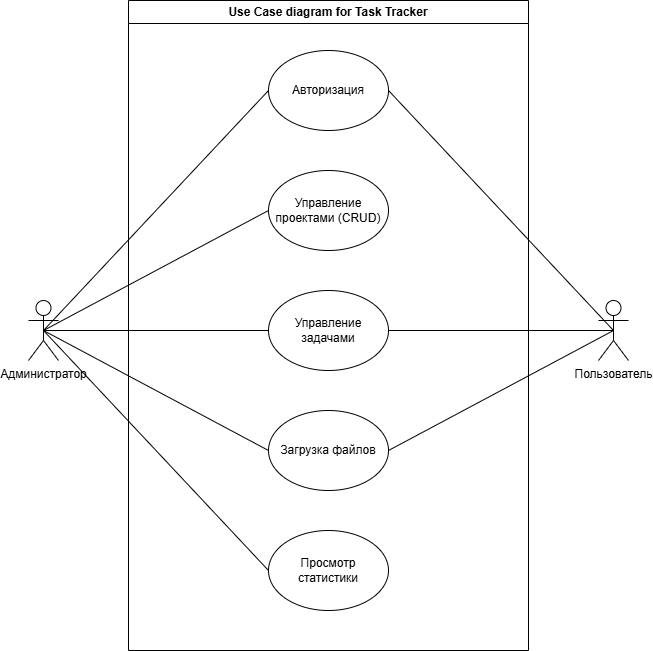
\includegraphics[width=0.8\textwidth]{images/use_case.png}
    \caption{Диаграмма вариантов использования системы}
    \label{fig:usecase}
\end{figure}

\clearpage

\subsection{Проектирование модели данных}

Проектирование базы данных веб-приложения осуществлялось в два этапа: разработка логической и физической схем. На рисунке \ref{fig:er_diagram} представлена ER-диаграмма, иллюстрирующая связи между основными объектами системы.

\begin{figure}[h!]
    \centering
    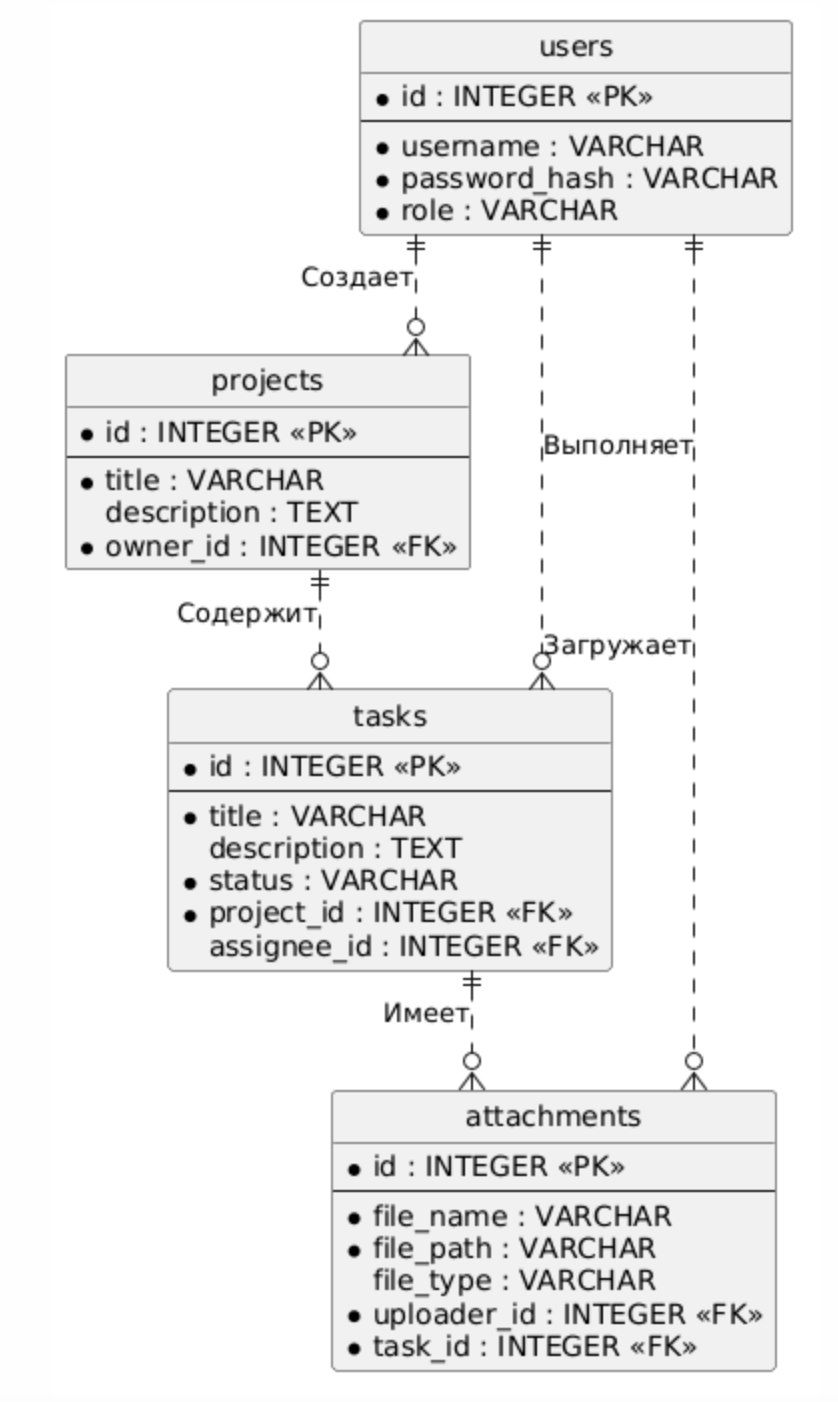
\includegraphics[width=0.45\textwidth]{images/er_diagram.png}
    \caption{ER-диаграмма базы данных}
    \label{fig:er_diagram}
\end{figure}

\textbf{Логическая схема базы данных} включает четыре основные сущности: \texttt{users} (Пользователи), \texttt{projects} (Проекты), \texttt{tasks} (Задачи) и \texttt{attachments} (Вложения). 

\textbf{Физическая схема базы данных} описывает реализацию таблиц в СУБД с указанием типов данных и ограничений. Структуры разработанных таблиц представлены в таблицах 2.1 --- 2.4.

\begin{table}[h!]
\centering
\small
\caption{Структура таблицы пользователей (users)}
\label{tab:users_db}
\begin{tabular}{|p{0.2\textwidth}|p{0.25\textwidth}|p{0.45\textwidth}|}
\hline
\textbf{Поле} & \textbf{Тип данных} & \textbf{Ограничения и описание} \\ \hline
id & INTEGER & PRIMARY KEY \\ \hline
username & VARCHAR(50) & UNIQUE, NOT NULL \\ \hline
password\_hash & VARCHAR(128) & NOT NULL (хэш пароля) \\ \hline
role & VARCHAR(20) & DEFAULT 'user' \\ \hline
\end{tabular}

\vspace{0.5cm} % Небольшой фиксированный отступ

\caption{Структура таблицы проектов (projects)}
\label{tab:projects_db}
\begin{tabular}{|p{0.2\textwidth}|p{0.25\textwidth}|p{0.45\textwidth}|}
\hline
\textbf{Поле} & \textbf{Тип данных} & \textbf{Ограничения и описание} \\ \hline
id & INTEGER & PRIMARY KEY \\ \hline
title & VARCHAR(100) & NOT NULL \\ \hline
description & TEXT & NULL \\ \hline
owner\_id & INTEGER & FOREIGN KEY $\rightarrow$ users.id \\ \hline
\end{tabular}

\vspace{0.5cm}

\caption{Структура таблицы задач (tasks)}
\label{tab:tasks_db}
\begin{tabular}{|p{0.2\textwidth}|p{0.25\textwidth}|p{0.45\textwidth}|}
\hline
\textbf{Поле} & \textbf{Тип данных} & \textbf{Ограничения и описание} \\ \hline
id & INTEGER & PRIMARY KEY \\ \hline
title & VARCHAR(100) & NOT NULL \\ \hline
description & TEXT & NULL (Детальное описание задачи) \\ \hline
status & VARCHAR(20) & DEFAULT 'pending' \\ \hline
project\_id & INTEGER & FOREIGN KEY $\rightarrow$ projects.id \\ \hline
assignee\_id & INTEGER & FOREIGN KEY $\rightarrow$ users.id \\ \hline
\end{tabular}

\vspace{0.5cm}

\caption{Структура таблицы вложений (attachments)}
\label{tab:attachments_db}
\begin{tabular}{|p{0.2\textwidth}|p{0.25\textwidth}|p{0.45\textwidth}|}
\hline
\textbf{Поле} & \textbf{Тип данных} & \textbf{Ограничения и описание} \\ \hline
id & INTEGER & PRIMARY KEY \\ \hline
file\_name & VARCHAR(255) & NOT NULL (Оригинальное имя) \\ \hline
file\_path & VARCHAR(255) & NOT NULL (Путь на сервере) \\ \hline
file\_type & VARCHAR(20) & NULL (Тип: pdf, docx и др.) \\ \hline
uploader\_id & INTEGER & FOREIGN KEY $\rightarrow$ users.id \\ \hline
task\_id & INTEGER & FOREIGN KEY $\rightarrow$ tasks.id \\ \hline
\end{tabular}
\end{table}

\clearpage

\subsection{Разработка макетов страниц}

Для обеспечения высокого уровня пользовательского опыта (UX) интерфейс приложения спроектирован в минималистичном стиле. Для разгрузки основной таблицы проектов функции просмотра деталей задачи и загрузки файлов были вынесены в отдельные модальные окна.

На рисунке \ref{fig:wireframe1} представлен макет панели управления (дашборда), а на рисунке \ref{fig:wireframe2} --- макет детальной страницы проекта с таблицей задач.

\begin{figure}[h!]
    \centering
    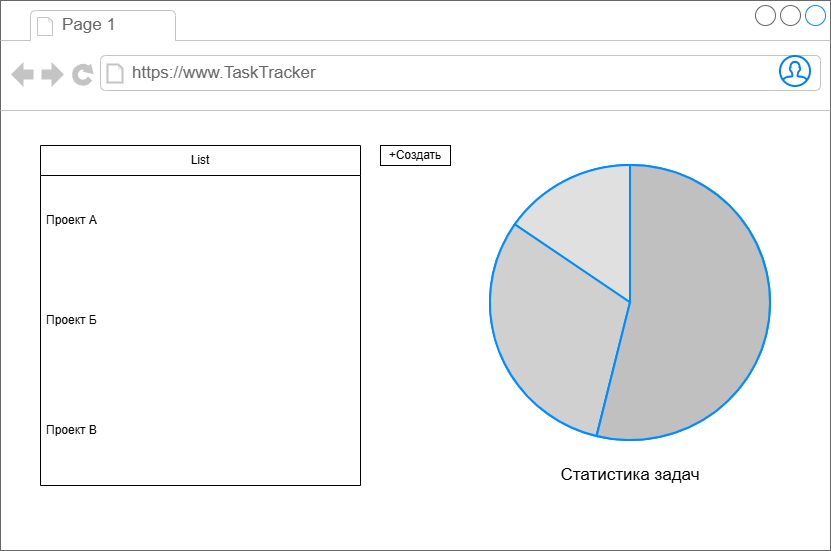
\includegraphics[width=0.85\textwidth]{images/wireframe1.png}
    \caption{Макет главной панели управления (Дашборд)}
    \label{fig:wireframe1}
\end{figure}

\begin{figure}[h!]
    \centering
    
\includegraphics[width=0.85\textwidth]{images/wireframe2.png}
    \caption{Макет страницы проекта со списком задач}
    \label{fig:wireframe2}
\end{figure}

\clearpage

Для демонстрации структуры дополнительных окон ниже представлены фактические экранные формы реализованного веб-приложения, утвержденные в рамках проектирования интерфейса. На рисунках \ref{fig:modal_create_proj} --- \ref{fig:modal_edit_proj} представлены окна управления проектом.

\begin{figure}[h!]
    \centering
    \begin{minipage}{0.48\textwidth}
        \centering
        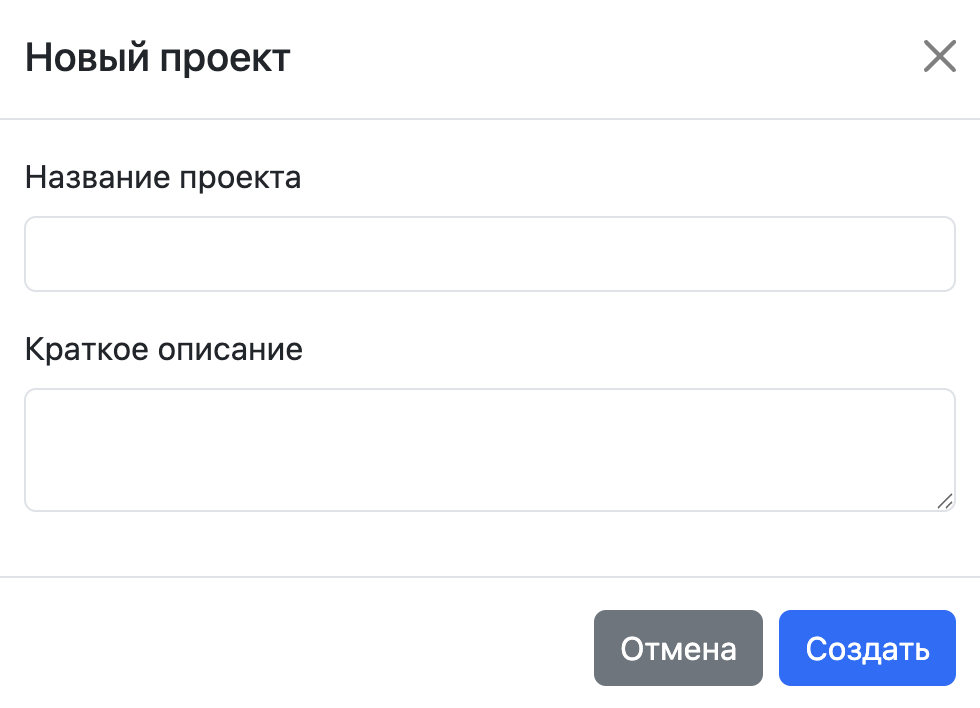
\includegraphics[width=\linewidth]{images/modal_create_proj.png}
        \caption{Окно создания проекта}
        \label{fig:modal_create_proj}
    \end{minipage}\hfill
    \begin{minipage}{0.48\textwidth}
        \centering
        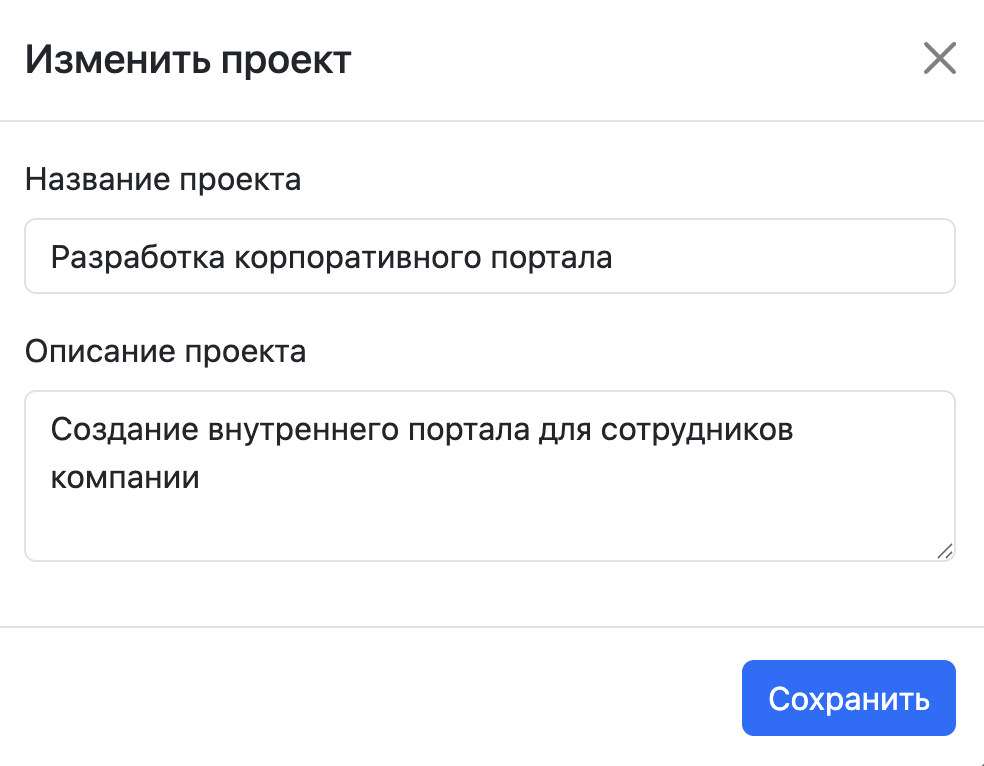
\includegraphics[width=\linewidth]{images/modal_edit_proj.png}
        \caption{Окно редактирования проекта}
        \label{fig:modal_edit_proj}
    \end{minipage}
\end{figure}

На рисунках \ref{fig:modal_create_task} --- \ref{fig:modal_edit_task} представлены окна создания и редактирования задач. На рисунке \ref{fig:modal_view_task} представлено окно просмотра, содержащее полное описание задачи и список прикрепленных файлов.

\begin{figure}[h!]
    \centering
    \begin{minipage}{0.48\textwidth}
        \centering
        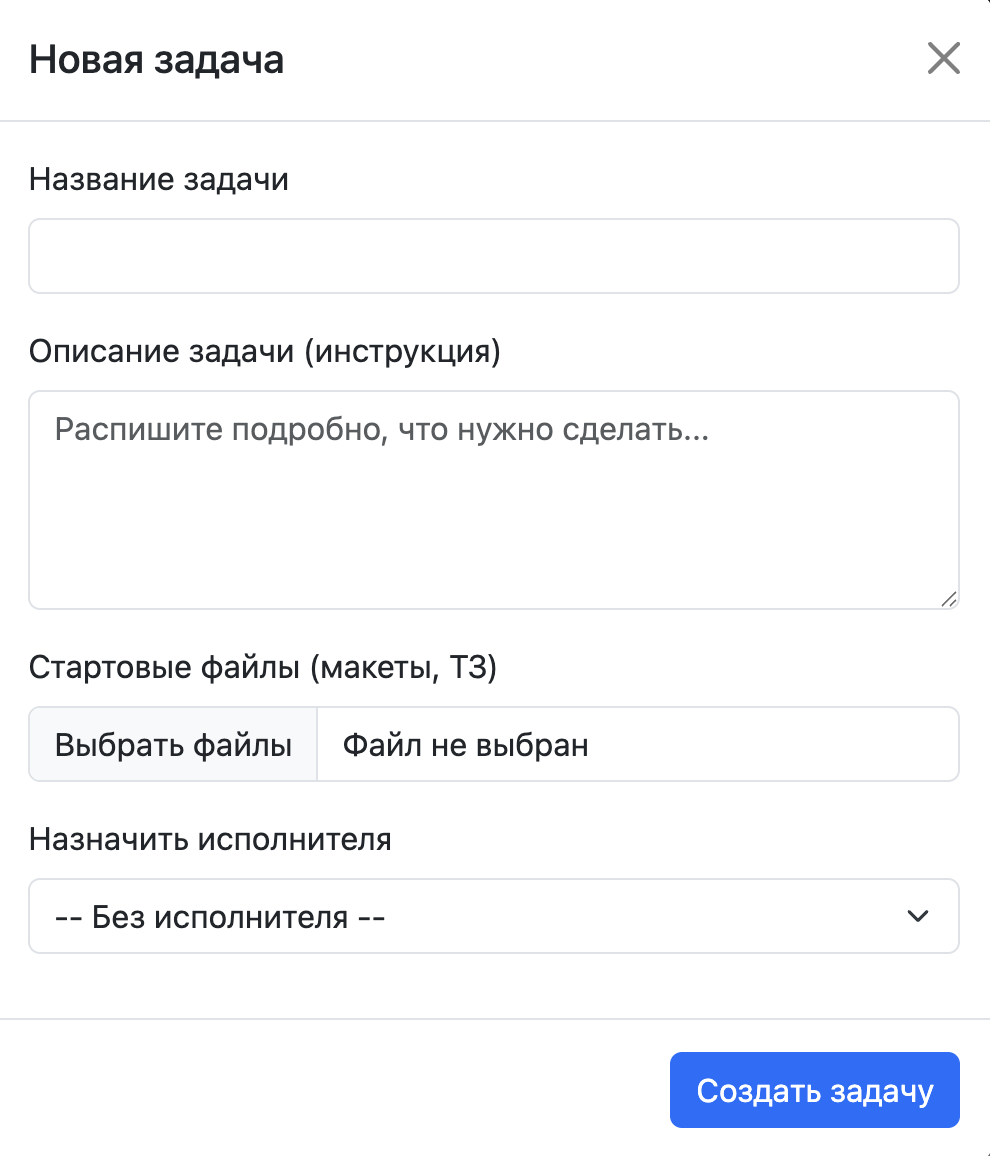
\includegraphics[width=\linewidth]{images/modal_create_task.png}
        \caption{Окно создания задачи}
        \label{fig:modal_create_task}
    \end{minipage}\hfill
    \begin{minipage}{0.48\textwidth}
        \centering
        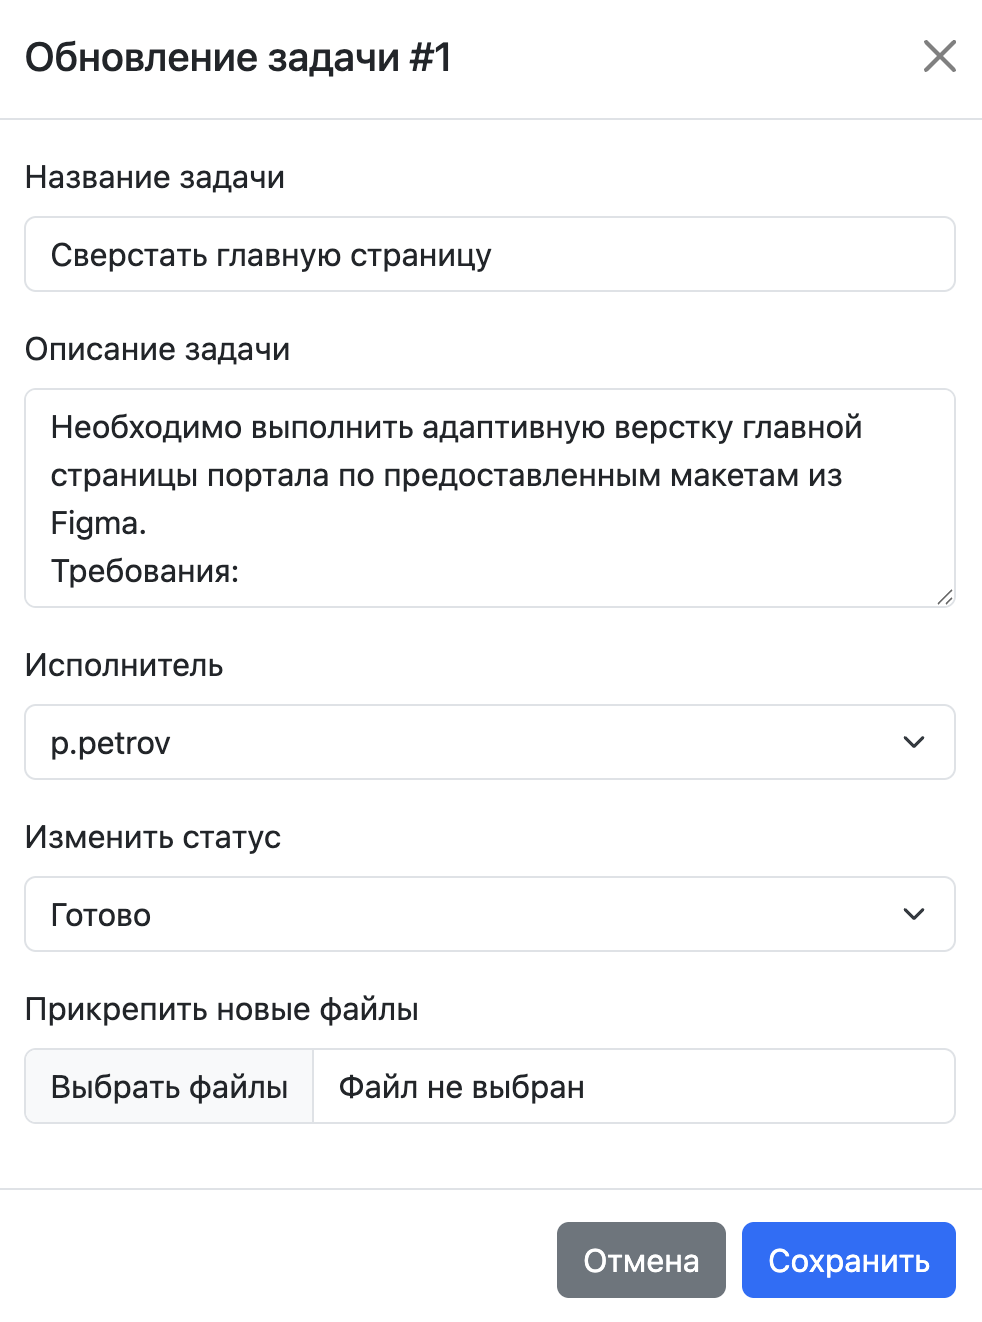
\includegraphics[width=\linewidth]{images/modal_edit_task.png}
        \caption{Окно редактирования задачи}
        \label{fig:modal_edit_task}
    \end{minipage}
\end{figure}

\begin{figure}[h!]
    \centering
    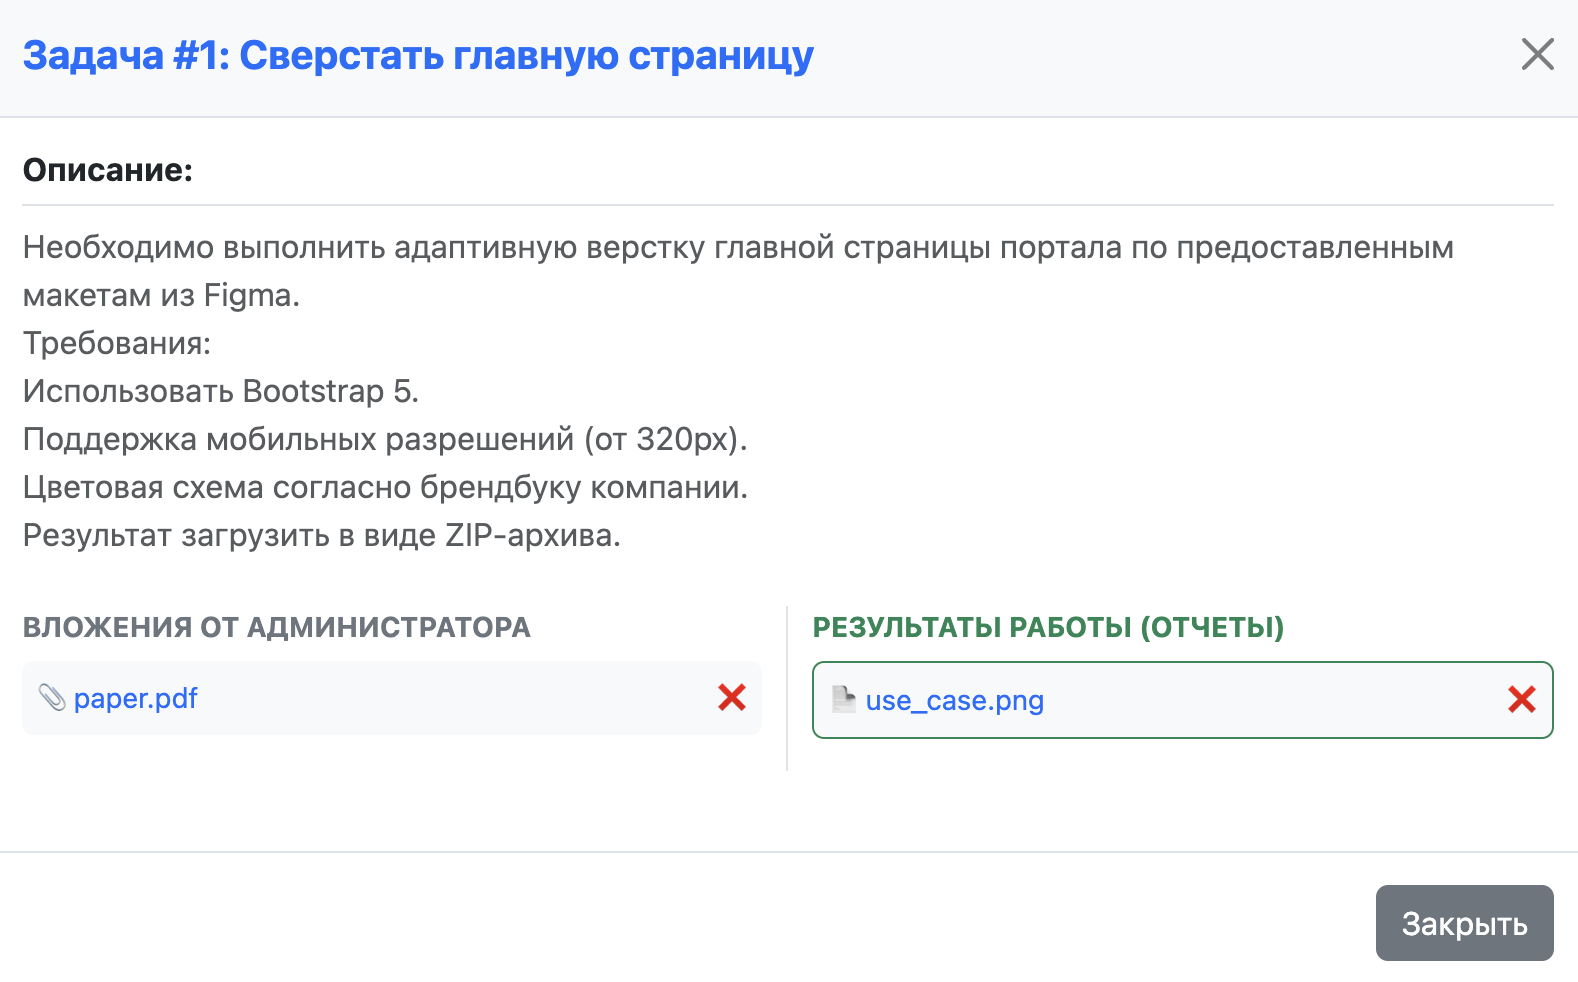
\includegraphics[width=0.85\textwidth]{images/modal_view_task.png}
    \caption{Окно просмотра описания и файлов задачи}
    \label{fig:modal_view_task}
\end{figure}